% SFDCT-HFF architecture — signal-processing paper style (monochrome, 3D tensor stacks + R-shape).
% Compile:  pdflatex fig_arch_sfdct_hff.tex      (standalone -> cropped PDF)
\documentclass[border=12pt]{standalone}
\usepackage{amsmath,amssymb}
\usepackage{tikz}
\usetikzlibrary{arrows.meta,calc,backgrounds,positioning}
\begin{document}
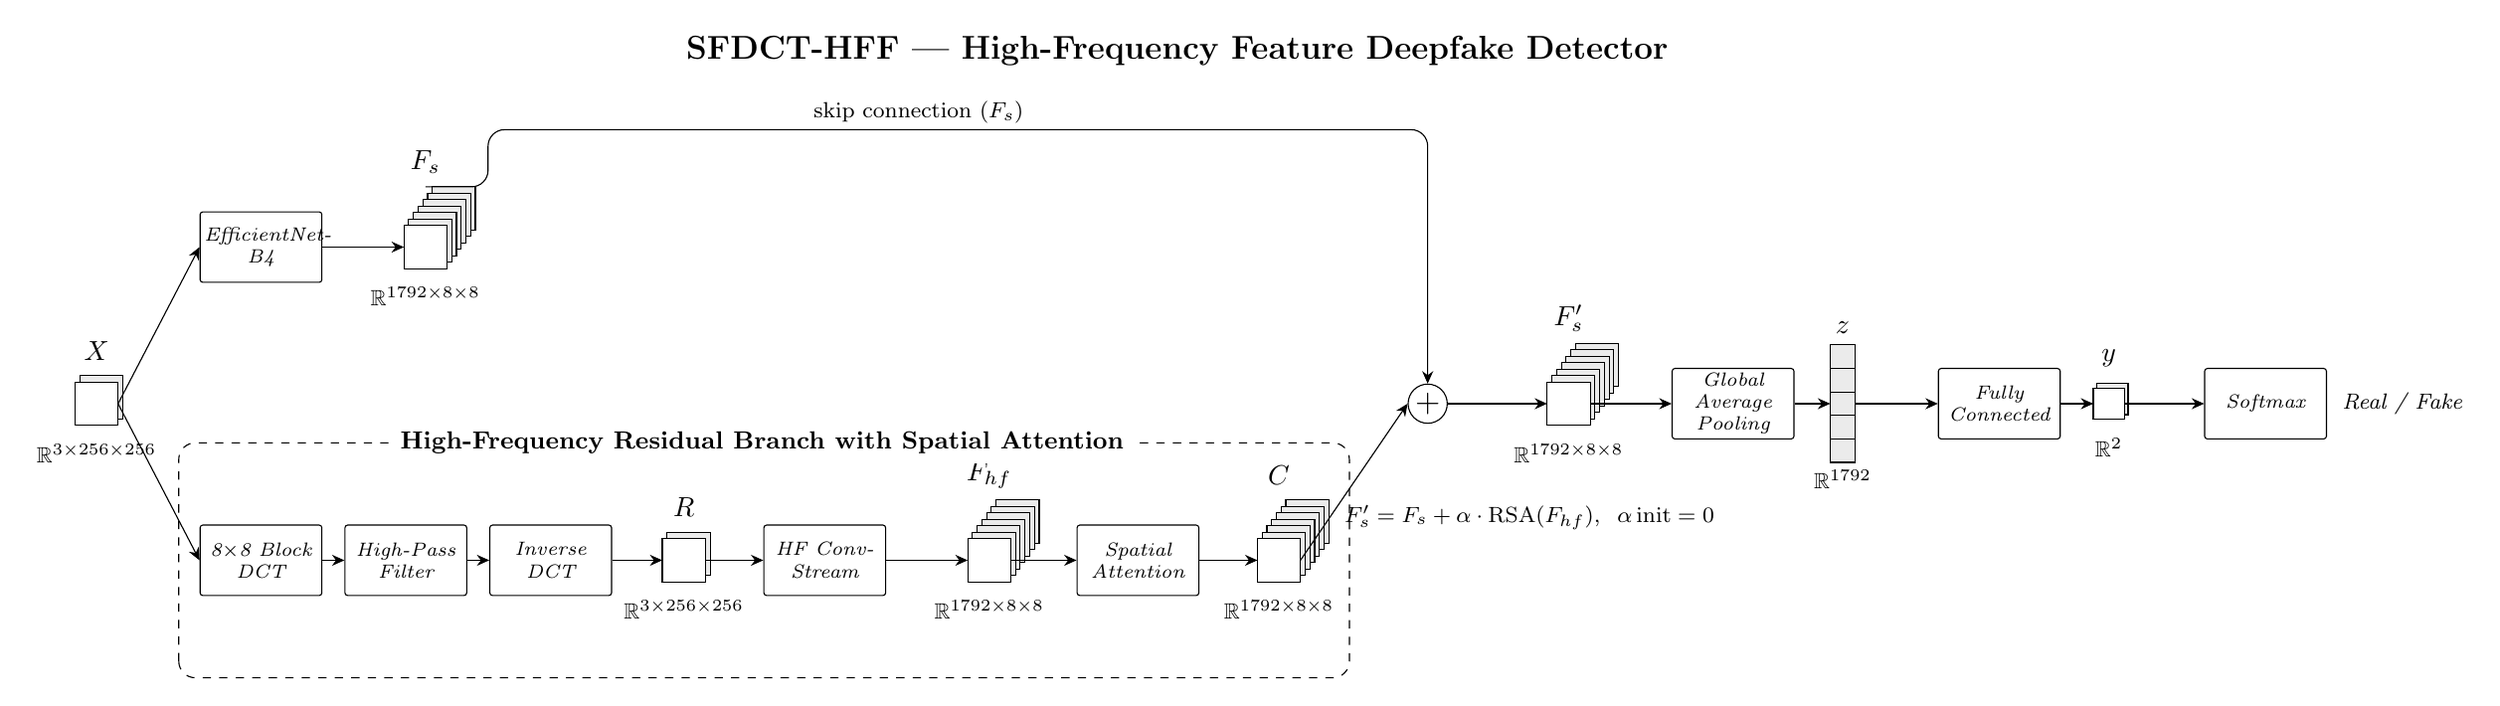
\begin{tikzpicture}[
  font=\small,
  op/.style={draw=black, thin, fill=white, rounded corners=1pt,
             text width=1.45cm, align=center, minimum height=0.9cm,
             inner sep=1.5pt, font=\scriptsize\itshape},
  arr/.style={-{Stealth[length=4.5pt,width=4pt]}, thin},
]
% ---- tensor-stack macro: #1 id #2 x #3 y #4 n #5 side #6 above #7 below ----
\newcommand{\stk}[7]{%
  \pgfmathsetmacro{\ss}{#5}\pgfmathsetmacro{\ox}{0.11*#5}\pgfmathsetmacro{\oy}{0.15*#5}%
  \foreach \i in {#4,...,1}{%
    \pgfmathtruncatemacro{\k}{\i-1}%
    \ifnum\i=1 \def\fc{white}\else \def\fc{black!8}\fi
    \pgfmathsetmacro{\xll}{#2 - \ss/2 + \k*\ox}\pgfmathsetmacro{\yll}{#3 - \ss/2 + \k*\oy}%
    \pgfmathsetmacro{\xur}{\xll + \ss}\pgfmathsetmacro{\yur}{\yll + \ss}%
    \draw[thin,fill=\fc] (\xll,\yll) rectangle (\xur,\yur);%
  }%
  \pgfmathtruncatemacro{\kn}{#4-1}%
  \pgfmathsetmacro{\ytop}{#3 + \ss/2 + \kn*\oy + 0.32}\pgfmathsetmacro{\ybot}{#3 - \ss/2 - 0.36}%
  \pgfmathsetmacro{\xw}{#2 - \ss/2}\pgfmathsetmacro{\xe}{#2 + \ss/2}\pgfmathsetmacro{\yn}{#3 + \ss/2 + \kn*\oy}\pgfmathsetmacro{\ysd}{#3 - \ss/2}%
  \node[font=\itshape] at (#2,\ytop) {#6};\node[font=\footnotesize] at (#2,\ybot) {#7};%
  \coordinate (#1-w) at (\xw,#3);\coordinate (#1-e) at (\xe,#3);\coordinate (#1-n) at (#2,\yn);\coordinate (#1-s) at (#2,\ysd);%
}
\newcommand{\vbar}[5]{%
  \draw[thin,fill=black!8] (#2-0.16,#3-0.75) rectangle (#2+0.16,#3+0.75);%
  \foreach \t in {1,...,4}{\pgfmathsetmacro{\yt}{#3-0.75+\t*0.3}\draw[thin] (#2-0.16,\yt)--(#2+0.16,\yt);}%
  \node[font=\itshape] at (#2,#3+0.97) {#4};\node[font=\footnotesize] at (#2,#3-0.97) {#5};%
  \coordinate (#1-w) at (#2-0.16,#3);\coordinate (#1-e) at (#2+0.16,#3);%
}

% ---- stacks ----
\stk{X}{0}{2}{2}{0.55}{$X$}{$\mathbb{R}^{3\times256\times256}$}
\stk{Fs}{4.2}{4}{7}{0.55}{$F_s$}{$\mathbb{R}^{1792\times8\times8}$}
\stk{R}{7.5}{0}{2}{0.55}{$R$}{$\mathbb{R}^{3\times256\times256}$}
\stk{Fhf}{11.4}{0}{7}{0.55}{$F_{hf}$}{$\mathbb{R}^{1792\times8\times8}$}
\stk{Cc}{15.1}{0}{7}{0.55}{$C$}{$\mathbb{R}^{1792\times8\times8}$}
\stk{Fsp}{18.8}{2}{7}{0.55}{$F_s'$}{$\mathbb{R}^{1792\times8\times8}$}
\vbar{z}{22.3}{2}{$z$}{$\mathbb{R}^{1792}$}
\stk{Yy}{25.7}{2}{2}{0.40}{$y$}{$\mathbb{R}^{2}$}

% ---- operations (full readable names) ----
\node[op] (B4)   at (2.1,4)  {EfficientNet-B4};
\node[op] (DCT)  at (2.1,0)  {8$\times$8 Block DCT};
\node[op] (HP)   at (3.95,0) {High-Pass\\Filter};
\node[op] (IDCT) at (5.8,0)  {Inverse DCT};
\node[op] (HFS)  at (9.3,0)  {HF Conv-\\Stream};
\node[op] (RSA)  at (13.3,0) {Spatial\\Attention};
\node[op] (GAP)  at (20.9,2) {Global\\Average Pooling};
\node[op] (FC)   at (24.3,2) {Fully\\Connected};
\node[op] (SM)   at (27.7,2) {Softmax};

% ---- gated residual add ----
\node[circle,draw,thin,inner sep=0pt,minimum size=0.5cm,font=\large] (plus) at (17.0,2) {$+$};
\node[font=\footnotesize,align=center] at (18.3,0.55)
  {$F_s' = F_s + \alpha\cdot \mathrm{RSA}(F_{hf}),\;\;\alpha\,\text{init}=0$};

% ---- edges ----
\draw[arr] (X-e) -- (B4.west);
\draw[arr] (X-e) -- (DCT.west);
\draw[arr] (B4.east) -- (Fs-w);
\draw[arr] (DCT.east) -- (HP.west);
\draw[arr] (HP.east)  -- (IDCT.west);
\draw[arr] (IDCT.east)-- (R-w);
\draw[arr] (R-e)      -- (HFS.west);
\draw[arr] (HFS.east) -- (Fhf-w);
\draw[arr] (Fhf-e)    -- (RSA.west);
\draw[arr] (RSA.east) -- (Cc-w);
% fusion
\draw[arr] (Cc-e) -- (plus.west);
% curved skip connection bypassing the module
\draw[arr,rounded corners=6pt] (Fs-n) -- ++(0.8,0) -- (5.0,5.5) -- (17.0,5.5) -- (plus.north);
\node[font=\footnotesize] at (10.5,5.72) {skip connection ($F_s$)};
% head
\draw[arr] (plus.east) -- (Fsp-w);
\draw[arr] (Fsp-e) -- (GAP.west);
\draw[arr] (GAP.east) -- (z-w);
\draw[arr] (z-e) -- (FC.west);
\draw[arr] (FC.east) -- (Yy-w);
\draw[arr] (Yy-e) -- (SM.west);
\node[font=\footnotesize,right=2pt of SM] {\itshape Real / Fake};

% ---- dashed module box + title ----
\begin{scope}[on background layer]
  \draw[dashed,rounded corners=6pt] (1.05,-1.5) rectangle (16.0,1.5);
\end{scope}
\node[fill=white,font=\bfseries\small] at (8.5,1.5)
  {High-Frequency Residual Branch with Spatial Attention};

% ---- figure title ----
\node[font=\bfseries\large] at (13.8,6.5)
  {SFDCT-HFF --- High-Frequency Feature Deepfake Detector};

\end{tikzpicture}
\end{document}
